\documentclass{article}

\usepackage[utf8]{inputenc}
\usepackage[T1]{fontenc}
\usepackage[greek,english]{babel}
\usepackage{alphabeta}
\usepackage{amsmath}
\usepackage{amssymb}
\usepackage{graphicx}
\usepackage{subcaption}
\usepackage{epstopdf}
\usepackage[margin=1in, paperwidth=7.5in,paperheight=10.5in]{geometry}
\usepackage{hyperref}
\usepackage{paracol}

\newcommand\course{ΗΡΥ 411}
\newcommand\courseName{Ενσωματωμένα Συστήματα Μικροεπεξεργατών}
\newcommand\semester{Χειμερινό 2020-2021}
\newcommand\assignmentNumber{Εργαστήριο 3}
\newcommand\studentName{Μαυρογιώργης Δημήτρης}                           
\newcommand\studentNumber{2016030016}

\title{\underline{\textbf{\assignmentNumber}}} 
\author{\textsc{\textbf{Όνομα:}}  \studentName\\
		\textsc{\textbf{ΑΜ:}}  \studentNumber\\
		\course \ - \courseName\\ 
		\textsc{Πολυτεχνείο Κρήτης}
		}
\date{\today}
\begin{document}
	\maketitle

\section*{Σκοπός}
	Σκοπός του τρίτου εργαστηρίου είναι η εξοικείωσή μας με τη σειριακή θύρα RS-232. Στο συγκεκριμένο εργαστήριο έχουμε δύο ανεξάρτητες διεργασίες που θα χρησιμοποιούν διαφορετικά Interrupts η κάθε μία. Η πρώτη διεργασία είναι αυτή που θα κάνει την ανανέωση των δεδομένων που εμφανίζουμε στα 7-segment LED, ενώ η δεύτερη θα επεξεργάζεται τα δεδομένα που λαμβάνονται και αποστέλονται από και προς τη σειριακή θύρα RS-232. 

\section*{Περιγραφή της υλοποίησης}
	Στο συγκεκριμενο εργαστήριο εκτος απο τις θύρες Α και C του προηγουμενου εργαστηριου χρησιμοποιήθηκαν και οι RXD, TXD για receive και transmit μέσω της σειριακής θύρα αντιστοιχα. Aρχικά, όπως λέει στο εγχειρίδιο του ATmega16, θα πρέπει να διασφαλίσουμε ότι τα Interrupts είναι απενεργοποιημένα και μόλις τελειώσει η αρχικοποίηση να ενεργοποιηθούν. Επιπλέον, για τη λειτουργία της σειρακής θύρας έπρεπε να ενεργοποιήσουμε το receive και transmit κάνοντας "1" τα bit RXEN και TXEN του καταχωρητή UCSRB. Για την ενεργοποίηση του rceive interrupt αρχικοποιήθηκε σε "1" και το bit RXCIE. \\
	
	\noindent
	Kατόπιν αρχικοποιήθηκε ο καταχωρητής UBRRL με την τιμή "0x41" ($65_{10}$) που είναι η τιμή BAUD για baud rate 9600 και συχνότητα 10 MHz. Τέλος, αφού έγινε "1" το bit URSEL του καταχωρητή UCSRC, για να μπορέσουμε να αρχικοποιήσουμε το συγκεκριμένο καταχωρητή και όχι το UBRR, τέθηκαν σε "1" τα bit UCSZ0 και UCSZ1 για να δηλώσουμε ότι έχουμε 8-bit κατά τη μετάδοση και λήψη. Τα bit UPM0 και UPM1 έμειναν "0", καθώς δεν έχουμε parity mode, ενώ το bit USBS έμεινε "0", επειδή έχουμε 1 stop bit.\\

	\noindent
	\textbf{Επεξήγηση Κώδικα} \\
	\noindent
	Αρχικά, στο data segment δεσμευουμε χωρο 4 byte για το OK<CR><LF>. Έπειτα δηλώθηκαν καποιες σταθερές που είναι οι ΗΕΧ τιμές των γραμμάτων εντολών A, T, C, N, O, K και ο χαρακτήρας X που χρησιμοποιήθηκε για να ξέρουμε κάθε φορά ότι ήρθε κάποιος αριθμός απο τη θύρα. Παράλληλα, δημιουργήθηκε μια ρουτίνα για clear της μνήμης, με την οποία αποθηκεύουμε την τιμή "0x0A" που σημαίνει ότι τα LED είναι σβηστά. Eπιπλέον, επειδή κατα την ανανέωση των 7-segment διβάζουμε από τη διεύθυνση "0x80" προς την "0x87" και η ανανέωση γίνεται από το LS Digit προς το MS Digit, χρειάζεται μια ρουτίνα για να κάνει shift τα δεδομένα, ώστε να εμφανίζονται σωστά. \\
	
	\pagebreak
	\noindent
	Όσον αφορά το handler για τη σειριακή θύρα και το receive των δεδομένων, η διεύθυνση μνήμης που βρίσκεται είναι η "0x16". Η υλοποίησή του είναι πολύ απλή, καθώς το μόνο που χρειάζεται να γίνει είναι να διαβάσουμε την τιμή του UDR σε ένα καταχωρητή και να ελέγχουμε με τον καταχωρητή r21, που έγινε define ως read\_char, ότι διαβάζονται σωστά οι εντολές και ανάλογα με την εντολή να κάνουμε την κατάλληλη ενέργεια και να στείλουμε OK<CR><LF>, μόλις λάβουμε και το <LF> της εντολής που εκτελέστηκε.
	
	
	\begin{figure}[h!]
		\centering
		\begin{subfigure}[t]{0.5\textwidth}
			\centering
			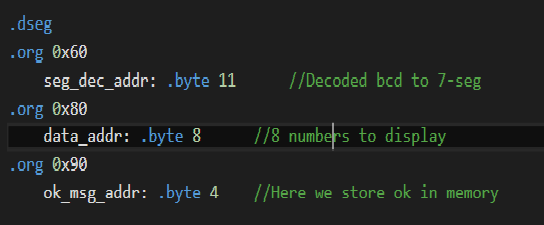
\includegraphics[height=3cm, width=\linewidth]{./results/lab3_dseg.png}
			\caption{Data segment}
		\end{subfigure}%
		~
		\begin{subfigure}[t]{0.5\textwidth}
			\centering
			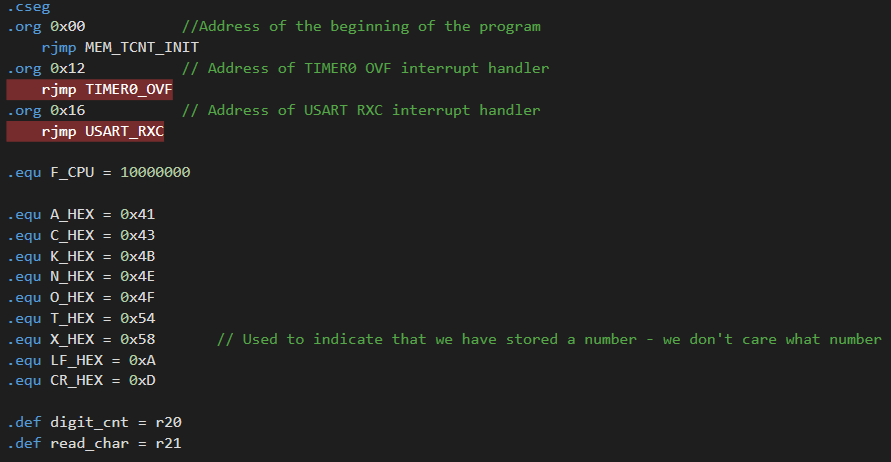
\includegraphics[height=3cm, width=\linewidth]{./results/lab3_cseg.png}
			\caption{Code segment - Definitions}
		\end{subfigure}
	
		\begin{subfigure}[t]{0.5\textwidth}
			\centering
			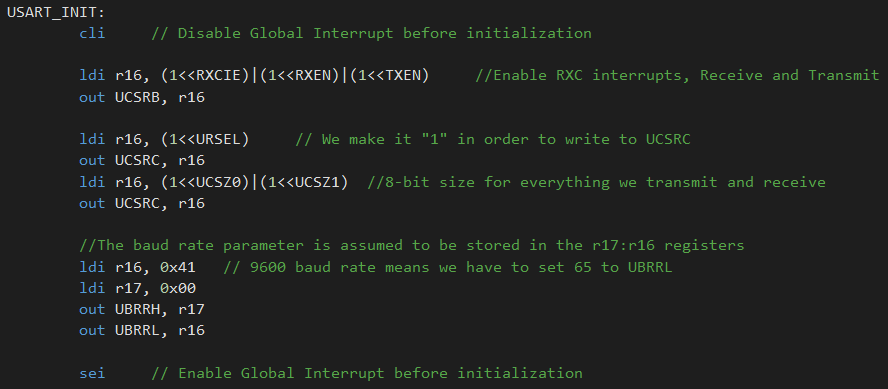
\includegraphics[height=3cm, width=\linewidth]{./results/lab3_usart_init.png}
			\caption{Usart Initialization}
		\end{subfigure}%
		~
		\begin{subfigure}[t]{0.5\textwidth}
			\centering
			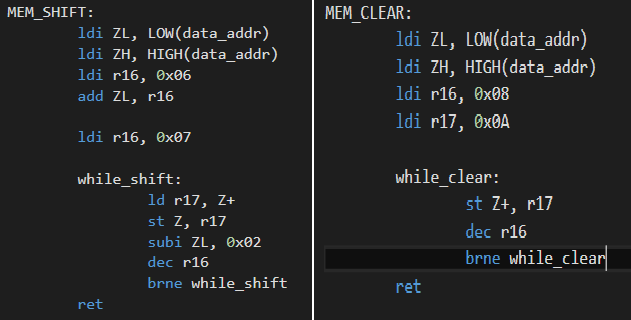
\includegraphics[height=3cm, width=\linewidth]{./results/lab3_clear_shift.png}
			\caption{Memory clear and data shift fucntion}
		\end{subfigure}	
	
		\begin{subfigure}[t]{0.5\textwidth}
			\centering
			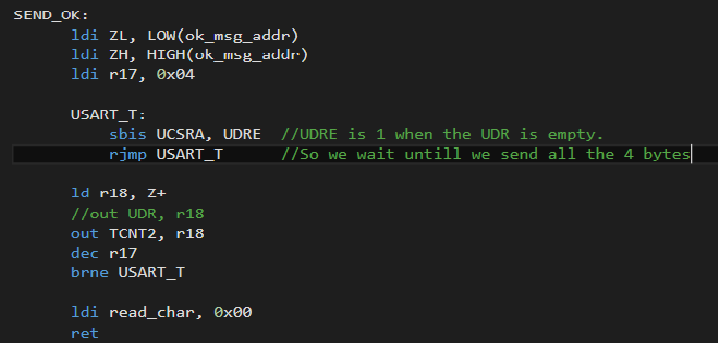
\includegraphics[height=3cm, width=\textwidth]{./results/lab3_send_ok.png}
			\caption{Function for sending OK}
		\end{subfigure}%
		~
		\begin{subfigure}[t]{0.5\textwidth}
			\centering
			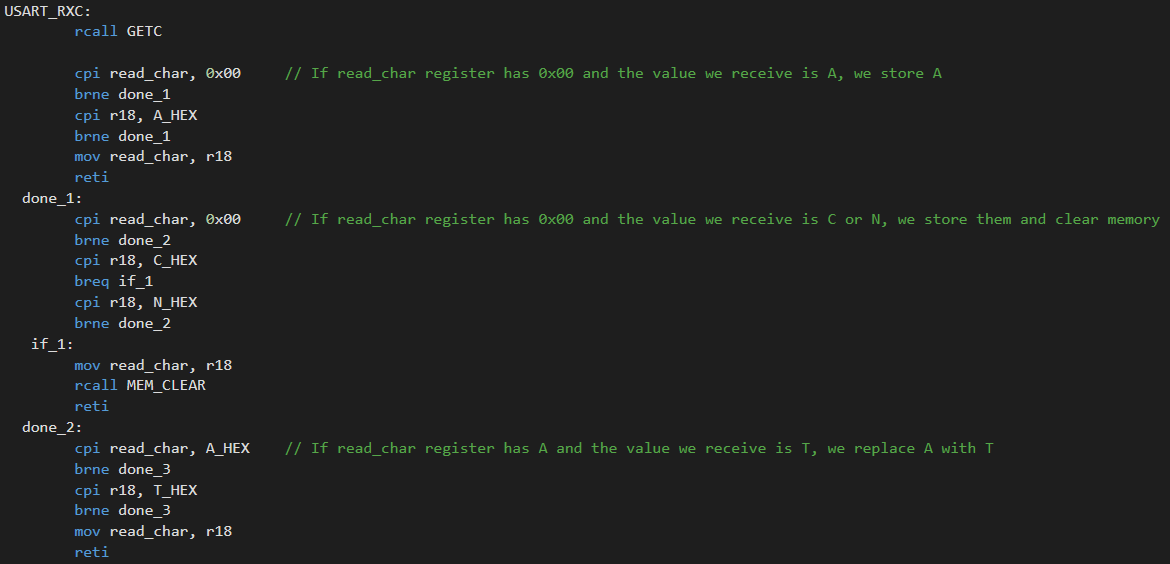
\includegraphics[height=3cm, width=\textwidth]{./results/lab3_usart_handler_a.png}
			\caption{Usart Interrupt Handler - A}
		\end{subfigure}	
	
		\begin{subfigure}[t]{0.5\textwidth}
			\centering
			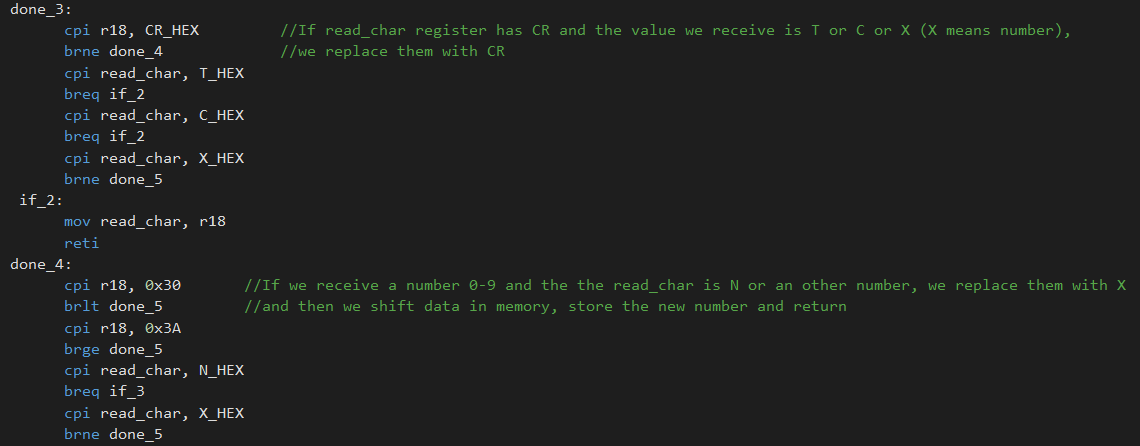
\includegraphics[height=3cm, width=\linewidth]{./results/lab3_usart_handler_b.png}
			\caption{Usart Interrupt Handler - B}
		\end{subfigure}%
		~
		\begin{subfigure}[t]{0.5\textwidth}
			\centering
			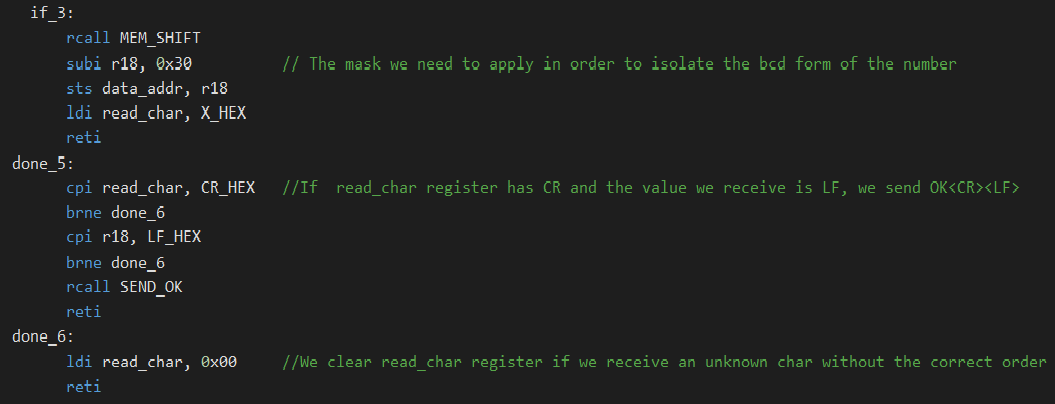
\includegraphics[height=3cm, width=\linewidth]{./results/lab3_usart_handler_c.png}
			\caption{Usart Interrupt Handler - C}
		\end{subfigure}	
	\end{figure}
	
	\noindent
	\textbf{Προσομοίωση Αποτελεσμάτων} \\
	\noindent
	Όπως φαίνεται και στην εικόνα (a) όλες οι αρχικοποιήσεις που περιγράφτηκαν παραπάνω γίνονται σωστά και για το USART και για τον TIMER/COUNTER0. Επιπλέον, Βλέπουμε ότι οι αποκωδικοποιήσεις των BCD, οι αριθμοί προς εμφάνιση και το OK<CR><LF> αποθηκεύονται στην SRAM. Στην επόμενη εικόνα παρατηρούμε ότι εκτελείται ο USART\_RXC handler και αποθηκεύεται ο αριθμός 0 που λαμβάνουμε μέσω του USART. Στην εικόνα (c) βλέπουμε ότι κάποια στιγμή εκτελείται ο TIMER0\_OVF handler και εμφανίζεται η τιμή 2 στο πρώτο digit. Έπειτα μετά από αρκετές εκτελέσεις του USART\_RXC handler, βλέπουμε ότι και οι οχτώ τιμές που λήφθηκαν μέσω του USART αποθηκεύονται σωστά στη μνήμη (εικόνα (e)). Στην ίδια εικόνα βλέπουμε ότι έρχεται για δεύτερη φορά ο TIMER0\_OVF handler και στην επόμενη εικόνα βλέπουμε ότι εμφανίζεται το 6 που αποθηκεύσαμε στη δεύτερη θέση μνήμης στο digit 2. Μόλις τελειώσει η λήψη και του <LF>, εκτελείται μόνο ο TIMER0\_OVF και γίνεται σωστά η ανανέωση των ψηφίων, όπως φαίνεται και στις επόμενες εικόνες. Στις εικόνες (g) και (h) φαίνεται ότι μετα την εμφάνιση του 6, εμφανίζεται το 5 στο ψηφίο 3 και στην επόμενη εκτέλεση εμφανίζεται το 4 στο digit 4 που είναι αποθηκευμένα στην τρίτη και τέταρτη θέση μνήμης αντίστοιχα. Συνεπώς, βλέπουμε ότι η λήψη και εμφάνιση των αριθμών γίνεται σωστά. Τέλος, όσον αφορά το OK<CR><LF> που στέλνουμε μετά από κάθε εντολή, φαίνεται ότι αποστέλονται σωστά τα byte OK<CR><LF> στο αρχείο lab3.log, αφού γίνεται η εγγραφή τους σε HEX μορφή σε αυτό το αρχείο.\\
	
	\begin{figure}[h!]
		\centering
		\begin{subfigure}[t]{0.5\textwidth}
			\centering
			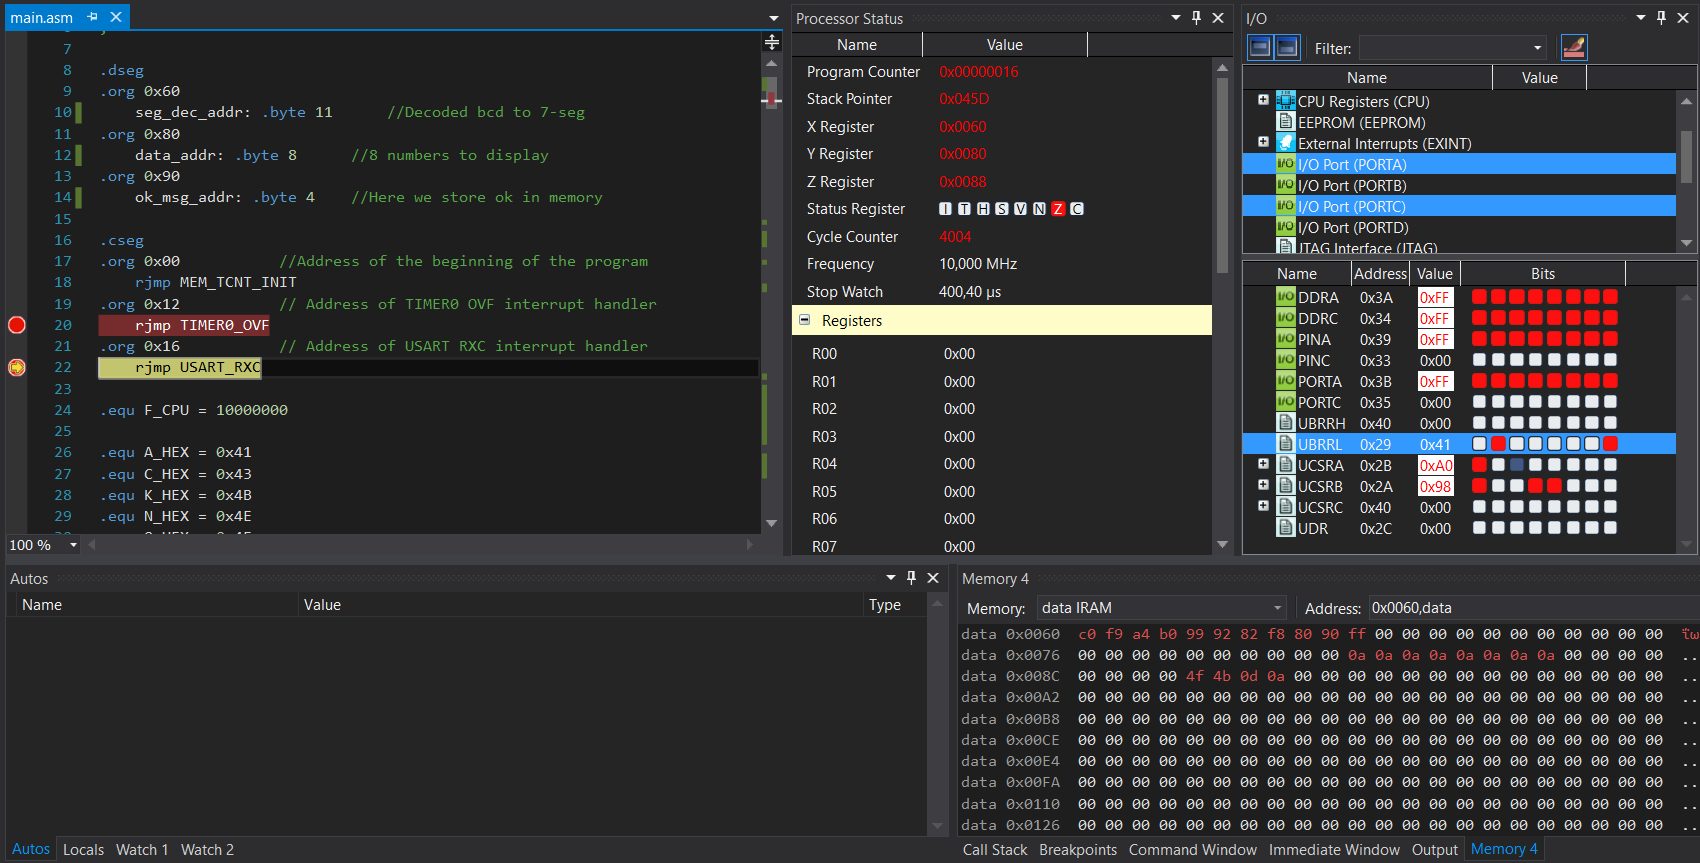
\includegraphics[height=3cm, width=\linewidth]{./results/lab3_sim_init.png}
			\caption{Results from Αtmel Studio 7 - Ιnitialization of registers and memory}
		\end{subfigure}%
		~
		\begin{subfigure}[t]{0.5\textwidth}
			\centering
			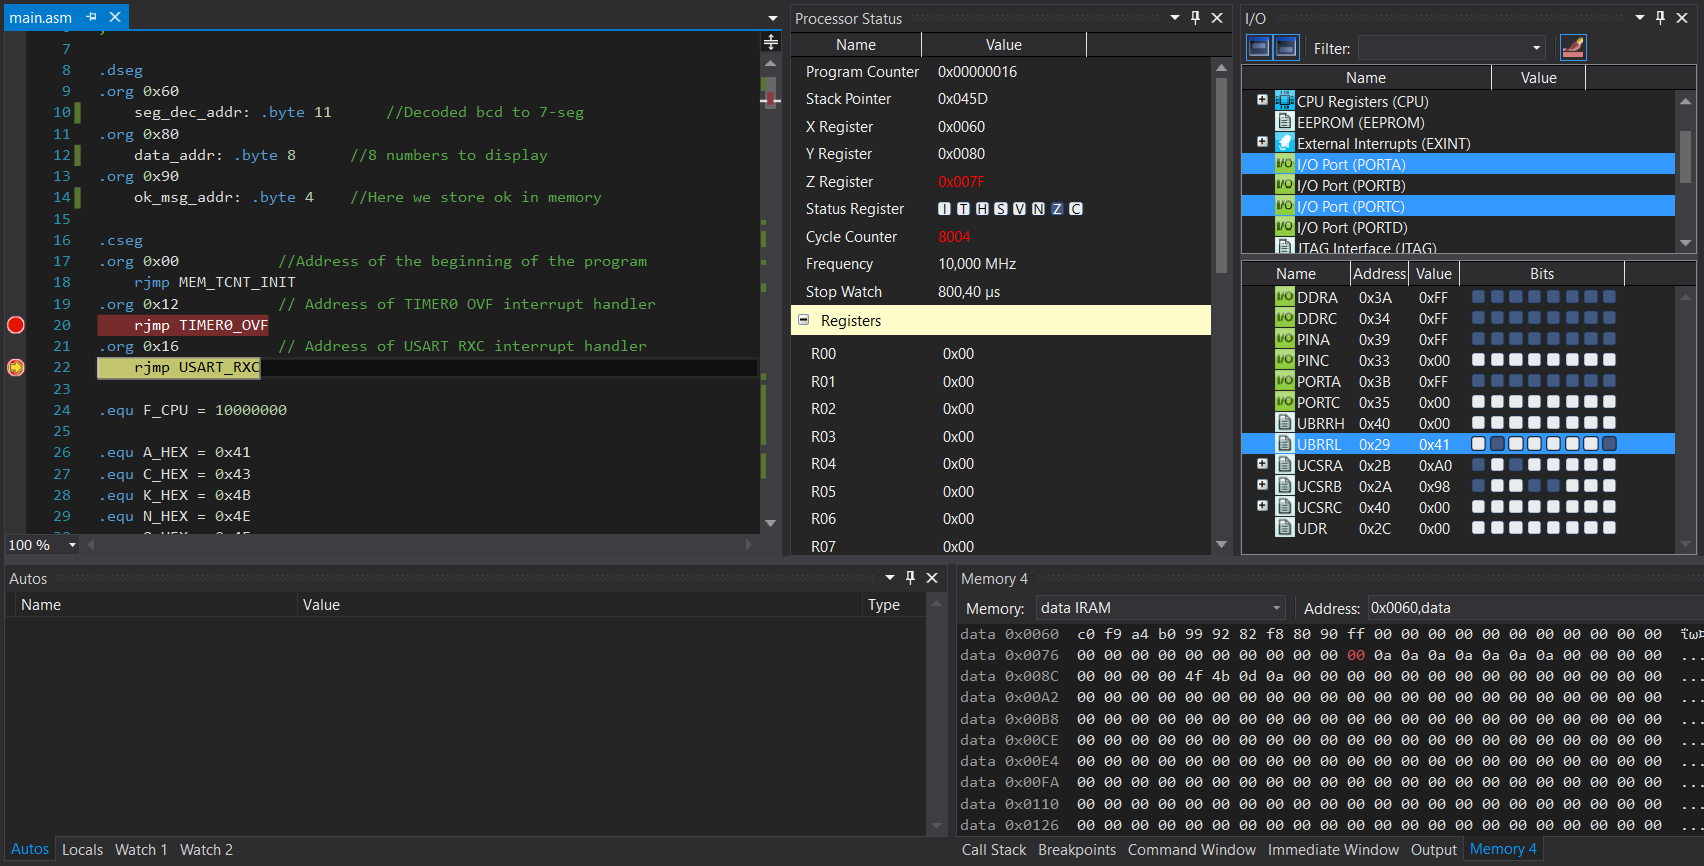
\includegraphics[height=3cm, width=\linewidth]{./results/lab3_num_instr_a.png}
			\caption{Results from Αtmel Studio 7 - Store of the first number}
		\end{subfigure}
		
		\begin{subfigure}[t]{0.5\textwidth}
			\centering
			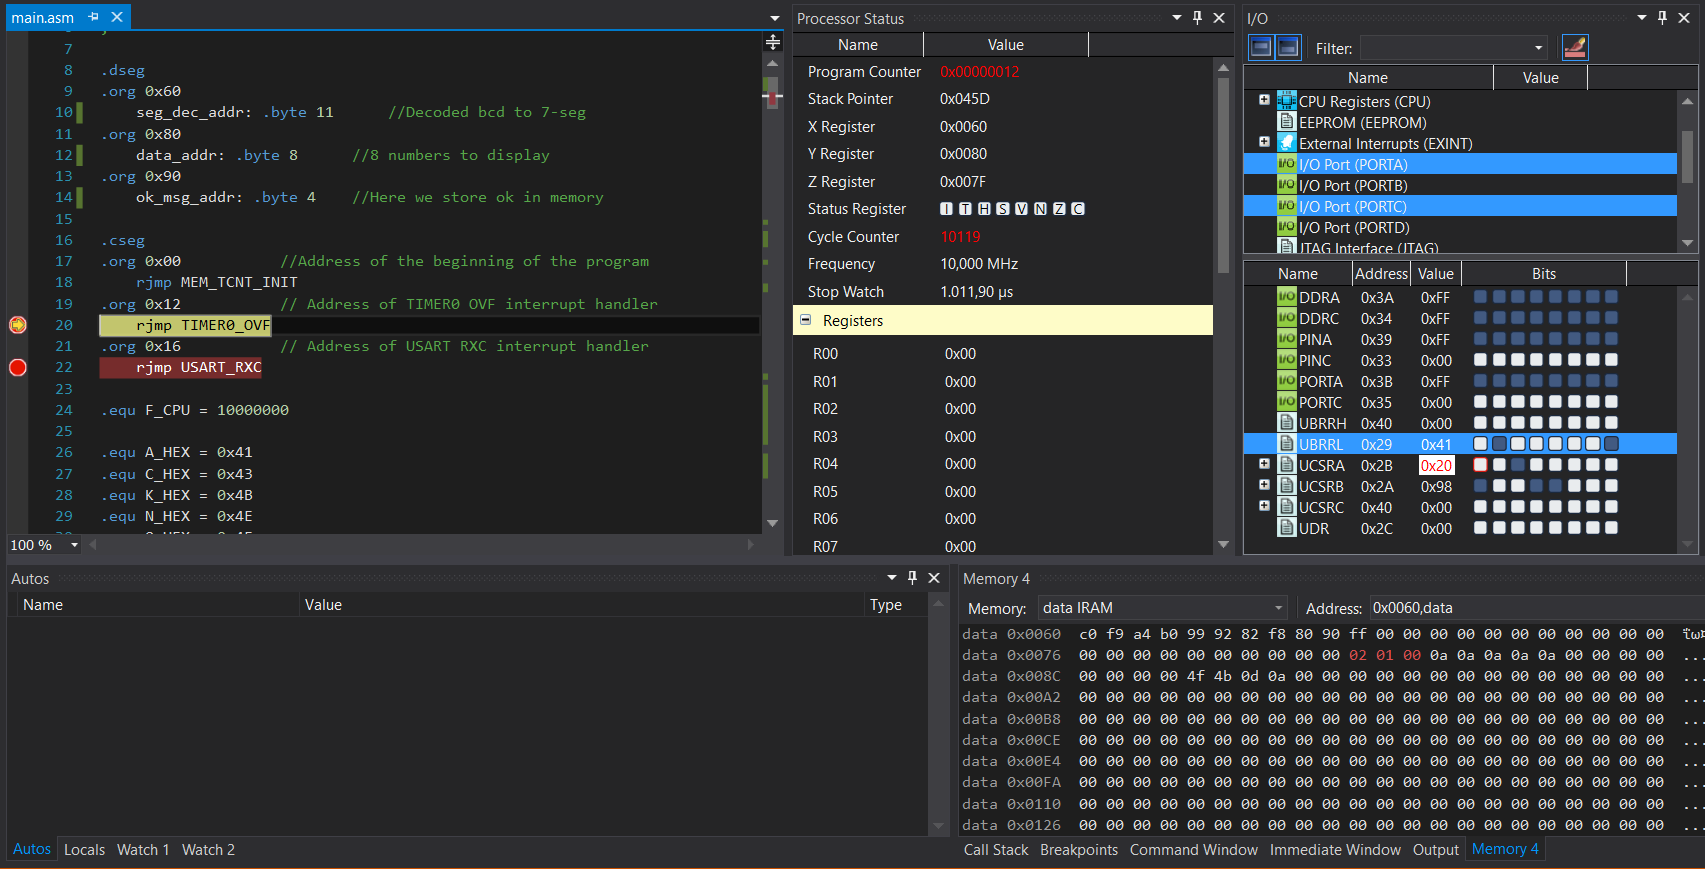
\includegraphics[height=3cm, width=\linewidth]{./results/lab3_num_instr_b.png}
			\caption{Results from Αtmel Studio 7 - Three number written and excecution of TIMER0 OVF handler}
		\end{subfigure}%
		~
		\begin{subfigure}[t]{0.5\textwidth}
			\centering
			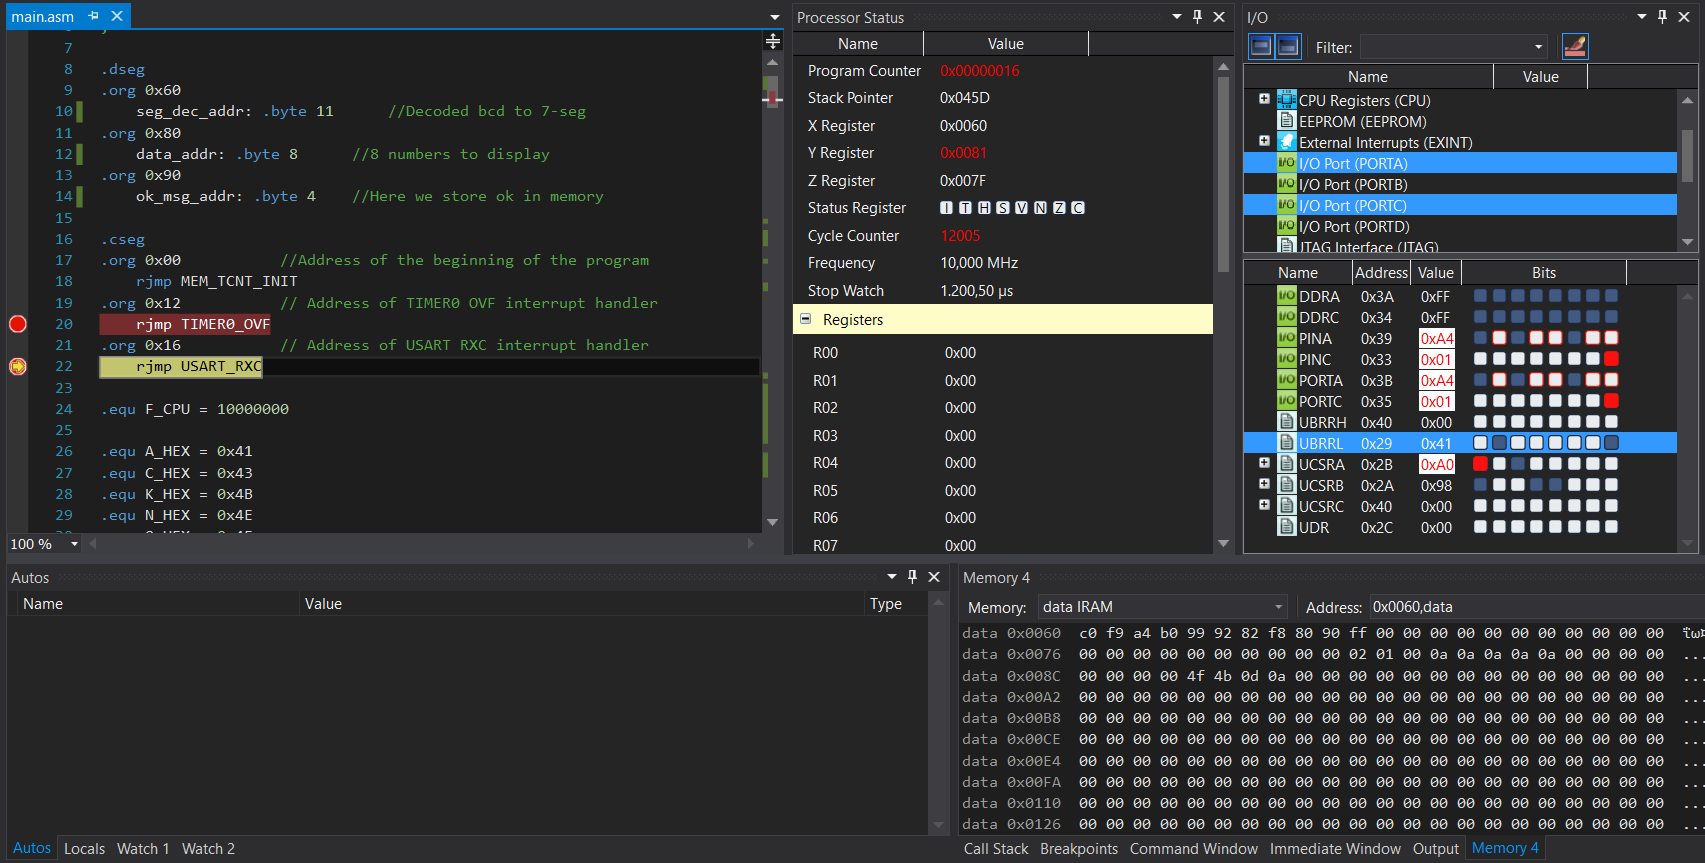
\includegraphics[height=3cm, width=\linewidth]{./results/lab3_num_instr_c.png}
			\caption{Results from Αtmel Studio 7 - After the execution of TIMER0 OVF handler}
		\end{subfigure}	
		
		\begin{subfigure}[t]{0.5\textwidth}
			\centering
			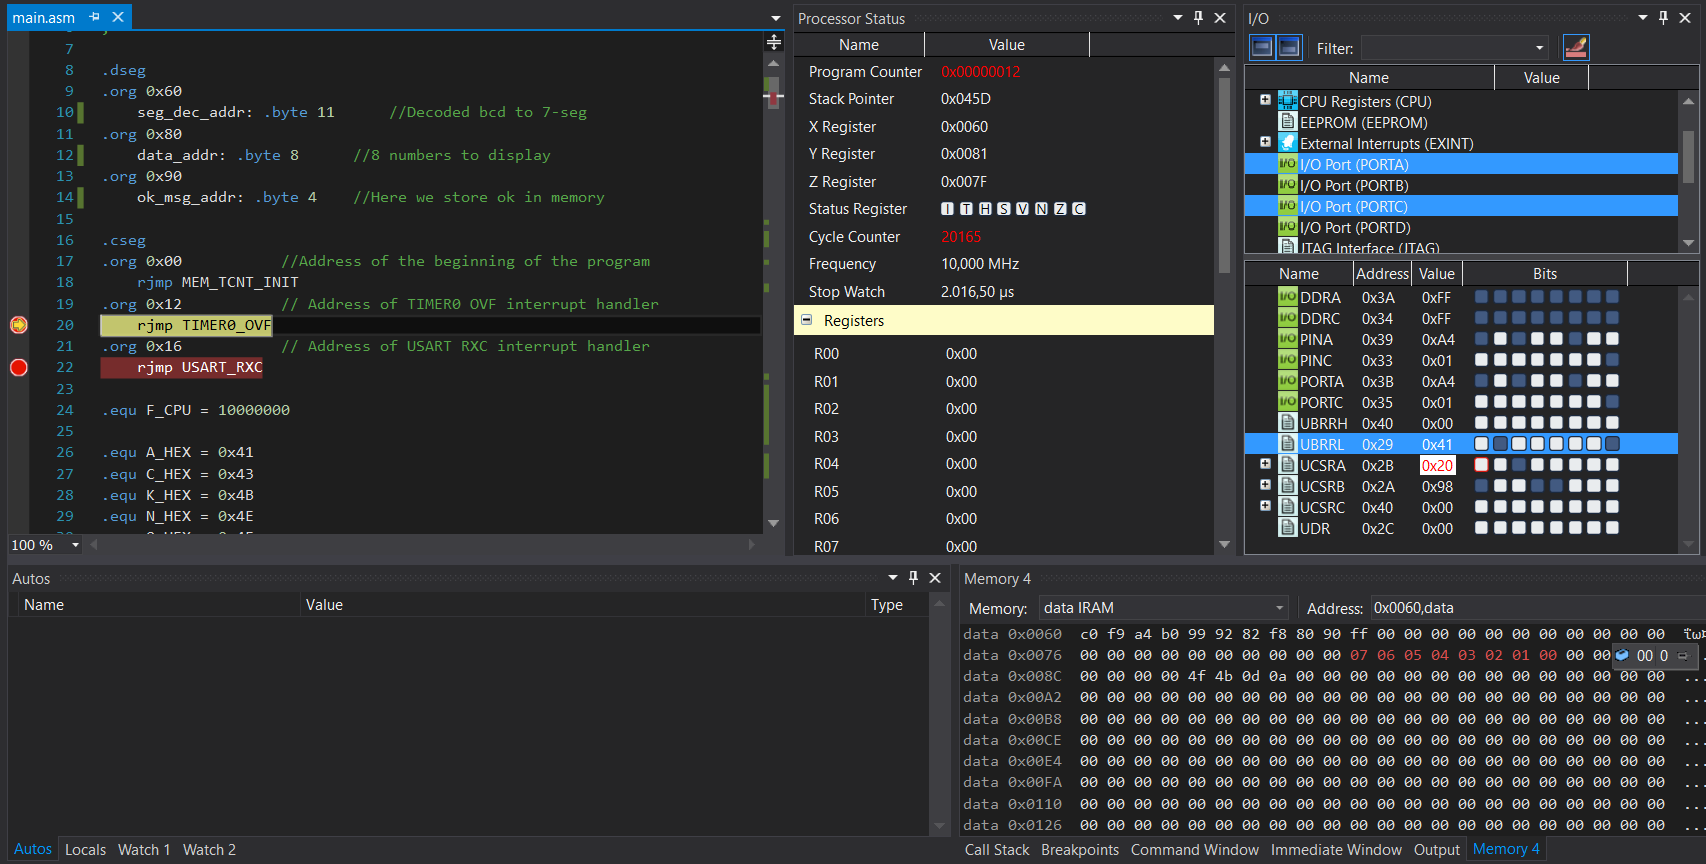
\includegraphics[height=3cm, width=\textwidth]{./results/lab3_num_instr_d.png}
			\caption{Results from Αtmel Studio 7 - All numbers stored and TIMER0 OVF handler is executed once again}
		\end{subfigure}%
		~
		\begin{subfigure}[t]{0.5\textwidth}
			\centering
			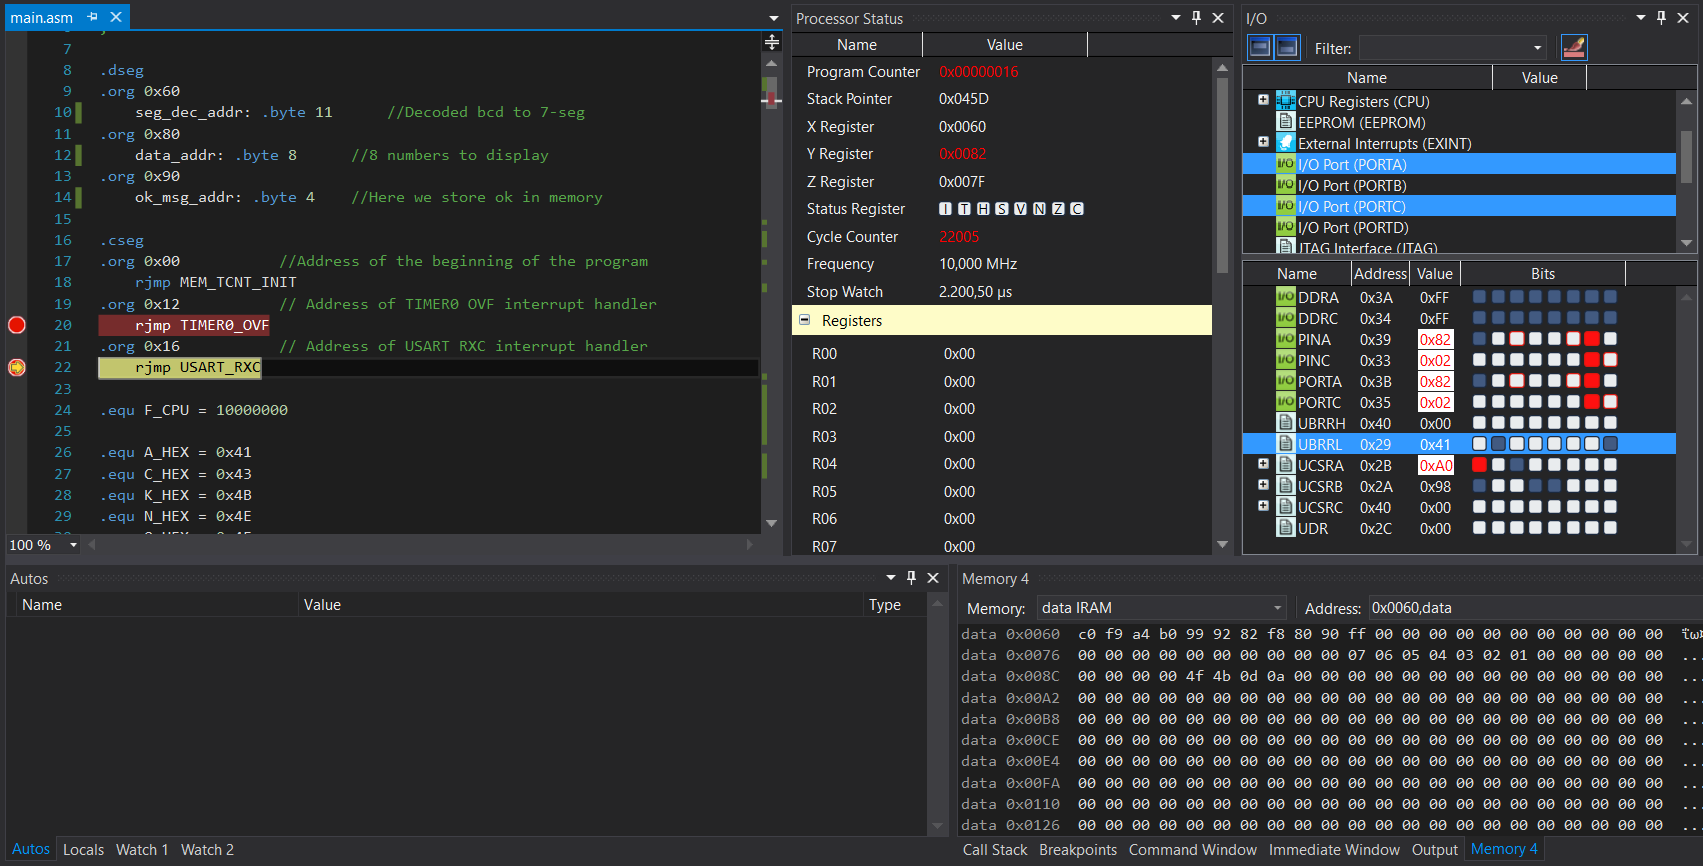
\includegraphics[height=3cm, width=\textwidth]{./results/lab3_num_instr_e.png}
			\caption{Results from Αtmel Studio 7 - After the second execution of TIMER0 OVF handler}
		\end{subfigure}	
		
		\begin{subfigure}[t]{0.5\textwidth}
			\centering
			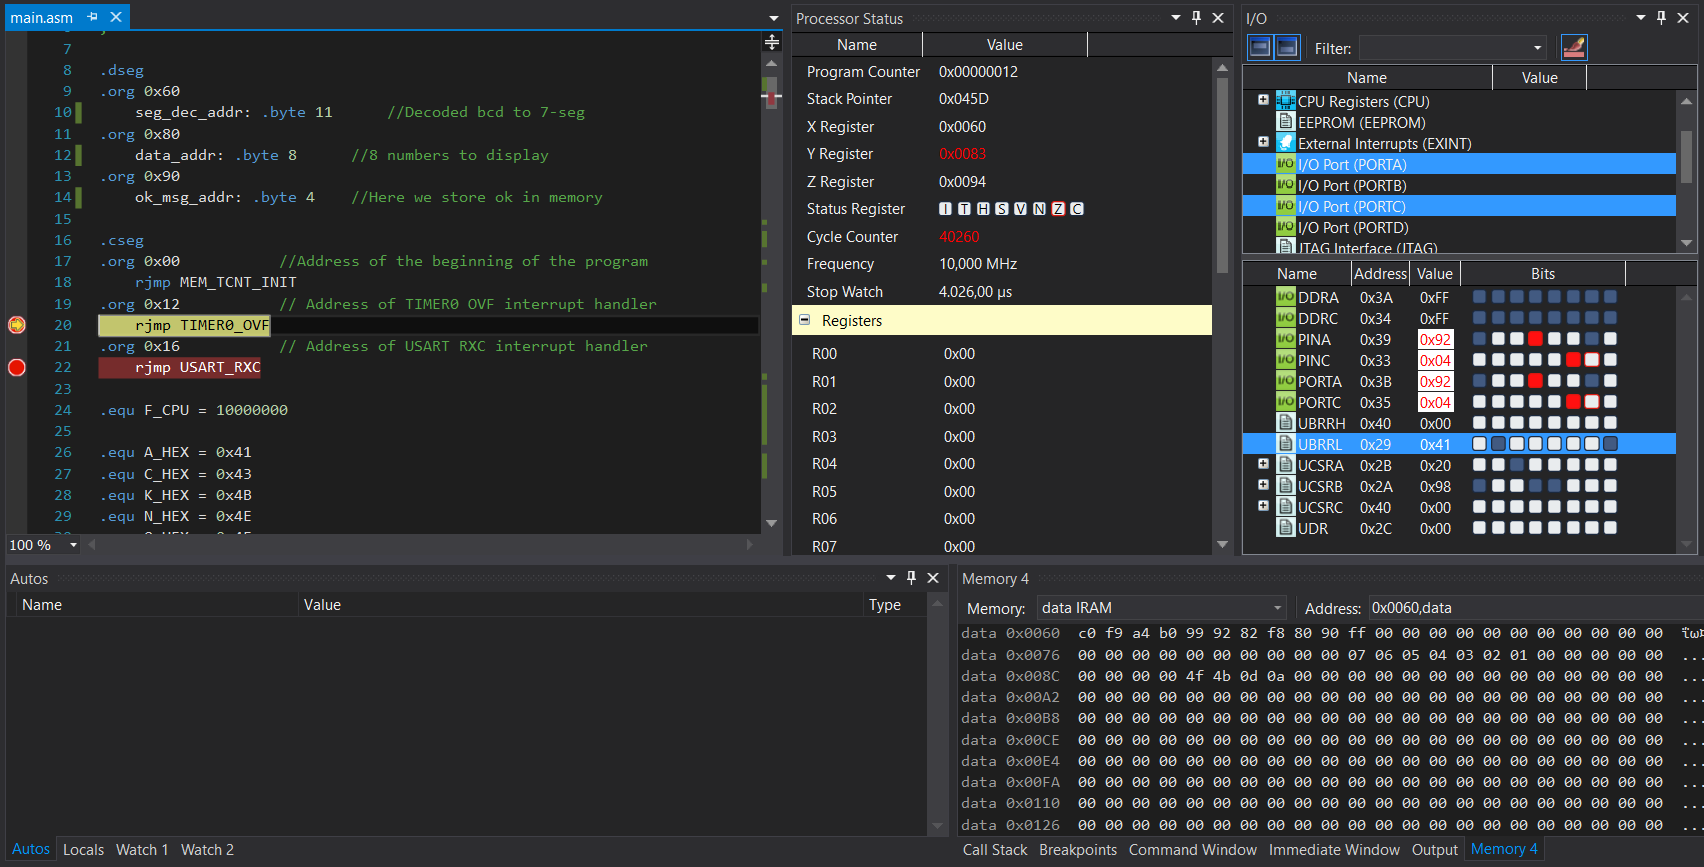
\includegraphics[height=3cm, width=\linewidth]{./results/lab3_num_instr_f.png}
			\caption{Results from Αtmel Studio 7 - After the third execution of TIMER0 OVF handler}
		\end{subfigure}%
		~
		\begin{subfigure}[t]{0.5\textwidth}
			\centering
			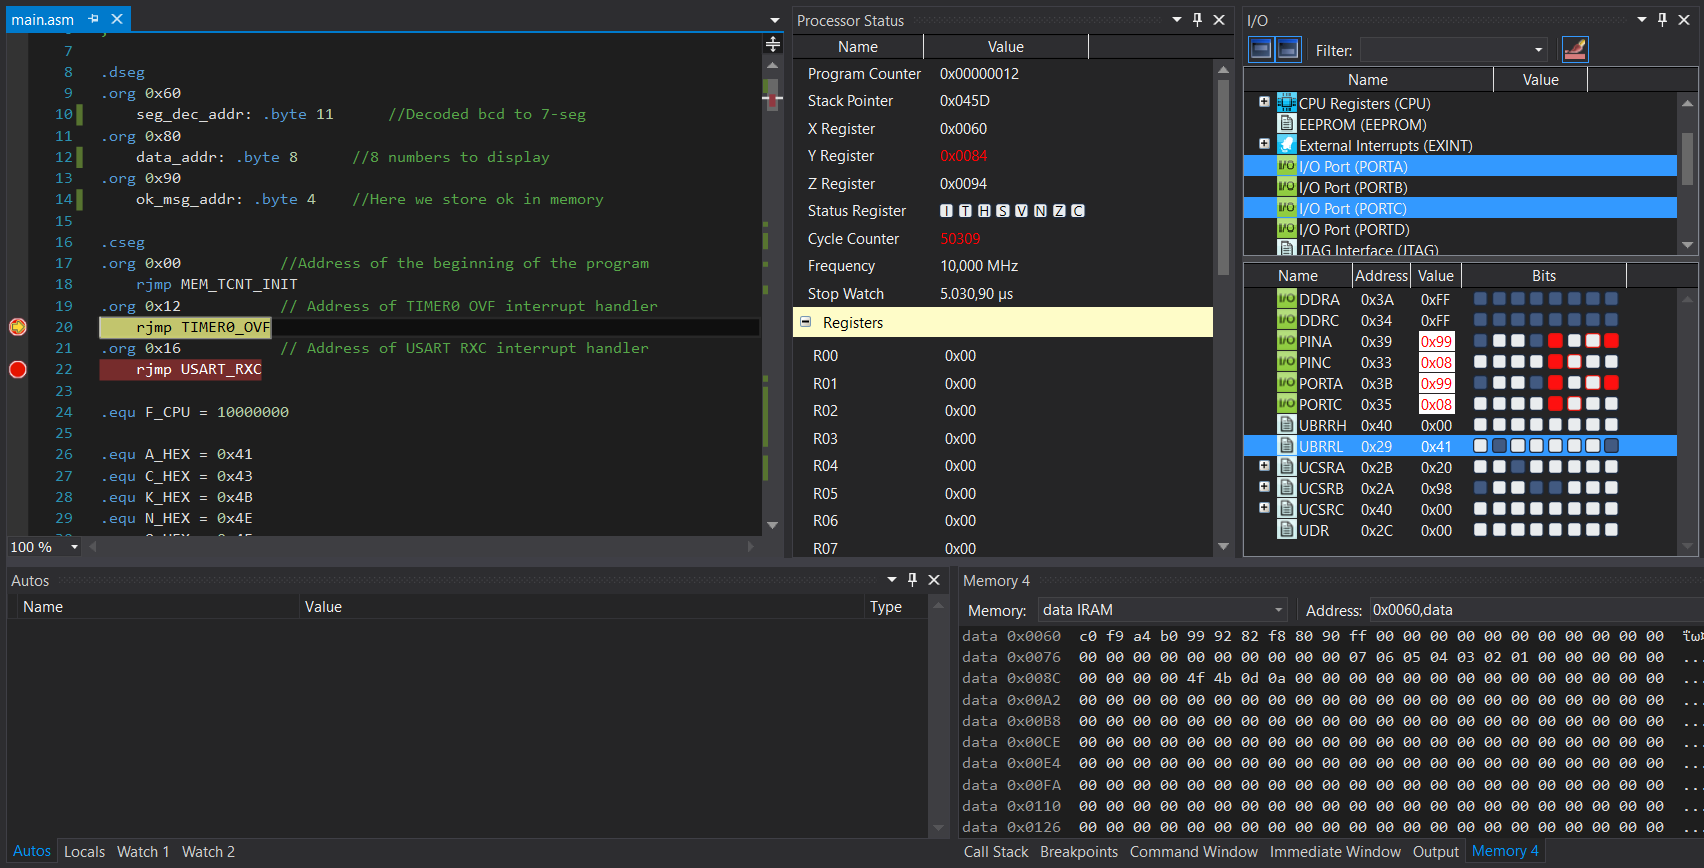
\includegraphics[height=3cm, width=\linewidth]{./results/lab3_num_instr_g.png}
			\caption{Results from Αtmel Studio 7 - After the forth execution of TIMER0 OVF handler}
		\end{subfigure}	
	\end{figure}
\end{document}
